\documentclass{beamer}
\usepackage[utf8]{inputenc}

\usetheme{Madrid}
\usecolortheme{default}
\usepackage{amsmath,amssymb,amsfonts,amsthm}
\usepackage{txfonts}
\usepackage{tkz-euclide}
\usepackage{listings}
\usepackage{adjustbox}
\usepackage{array}
\usepackage{tabularx}
\usepackage{gvv}
\usepackage{lmodern}
\usepackage{circuitikz}
\usepackage{tikz}
\usepackage{graphicx}

\setbeamertemplate{page number in head/foot}[totalframenumber]

\usepackage{tcolorbox}
\tcbuselibrary{minted,breakable,xparse,skins}



\definecolor{bg}{gray}{0.95}
\DeclareTCBListing{mintedbox}{O{}m!O{}}{%
  breakable=true,
  listing engine=minted,
  listing only,
  minted language=#2,
  minted style=default,
  minted options={%
    linenos,
    gobble=0,
    breaklines=true,
    breakafter=,,
    fontsize=\small,
    numbersep=8pt,
    #1},
  boxsep=0pt,
  left skip=0pt,
  right skip=0pt,
  left=25pt,
  right=0pt,
  top=3pt,
  bottom=3pt,
  arc=5pt,
  leftrule=0pt,
  rightrule=0pt,
  bottomrule=2pt,

  colback=bg,
  colframe=orange!70,
  enhanced,
  overlay={%
    \begin{tcbclipinterior}
    \fill[orange!20!white] (frame.south west) rectangle ([xshift=20pt]frame.north west);
    \end{tcbclipinterior}},
  #3,
}
\lstset{
    language=C,
    basicstyle=\ttfamily\small,
    keywordstyle=\color{blue},
    stringstyle=\color{orange},
    commentstyle=\color{green!60!black},
    numbers=left,
    numberstyle=\tiny\color{gray},
    breaklines=true,
    showstringspaces=false,
}
%------------------------------------------------------------
%This block of code defines the information to appear in the
%Title page
\title %optional
{4.7.14}
\date{september 2025}
%\subtitle{A short story}

\author % (optional)
{J.NAVYASRI- EE25BTECH11028}

\begin{document}

\frame{\titlepage}
\begin{frame}{Question:}
Find the distance of the plane 
2x - 3y + 4z - 6 = 0
from the origin.
\end{frame}

\begin{frame}{Solution:}
We want to find the distance of the plane 
\begin{equation}
2x - 3y + 4z - 6 = 0 \quad \text{(1)}
\end{equation} 
from the origin using the vector approach

\vspace{0.5em}
\textbf{Step 1: Identify the normal vector.}

The general equation of a plane is 
\begin{equation}
\mathbf{n} \cdot \mathbf{r} = D \quad \text{(2)}
\end{equation}
\end{frame}

\begin{frame}{Solution:}
where 
\begin{equation}
\mathbf{n} = \begin{pmatrix} A \\ B \\ C \end{pmatrix} \quad \text{(3)}
\end{equation} 
is the normal vector of the plane and $D$ is a constant. 

From the given plane ($2x - 3y + 4z = 6$), we have
\begin{equation}
\mathbf{n} = \begin{pmatrix} 2 \\ -3 \\ 4 \end{pmatrix}, \quad D = 6. \quad \text{(4)}
\end{equation}

\vspace{0.5em}
\textbf{Step 2: Distance formula.}

The distance of a point $\mathbf{r}_0$ from the plane is given by
\begin{equation}
\text{Distance} = \frac{|\mathbf{n} \cdot \mathbf{r}_0 - D|}{\|\mathbf{n}\|} \quad \text{(5)}.
\end{equation}
\end{frame}

\begin{frame}{Solution:}
For the origin, $\mathbf{r}_0 = \begin{pmatrix} 0 \\ 0 \\ 0 \end{pmatrix}$, so
\begin{equation}
\begin{split}
\text{Distance} &= \frac{|\mathbf{n} \cdot \mathbf{r}_0 - 6|}{\sqrt{2^2 + (-3)^2 + 4^2}} \\
&= \frac{|(2)(0) + (-3)(0) + (4)(0) - 6|}{\sqrt{4 + 9 + 16}} \\
&= \frac{|-6|}{\sqrt{29}} = \frac{6}{\sqrt{29}} \quad \text{(6)}.
\end{split}
\end{equation}

\vspace{0.5em}
\textbf{Answer:}
\begin{equation}
\boxed{\frac{6}{\sqrt{29}}} \quad \text{(7)}
\end{equation}
\end{frame}

\begin{frame}[fragile]
    \frametitle{Python Code}
    \begin{lstlisting}
import numpy as np
import matplotlib.pyplot as plt

# Plane coefficients: 2x - 3y + 4z - 6 = 0
a, b, c, d = 2, -3, 4, -6

# Denominator
den = a*a + b*b + c*c

# Origin
origin = np.array([0.0, 0.0, 0.0])

# Foot of perpendicular from origin to plane
foot = np.array([
    -a*d/den,
    -b*d/den,
    -c*d/den
])
\end{lstlisting}
\end{frame}


\begin{frame}[fragile]
    \frametitle{Python Code}
    \begin{lstlisting}
# Distance from origin to plane
distance = abs(d) / np.sqrt(den)

print("Foot of perpendicular:", foot)
print("Distance:", distance)

# Create grid for plane
grid_size = 3.0
num = 40
X = np.linspace(foot[0] - grid_size, foot[0] + grid_size, num)
Y = np.linspace(foot[1] - grid_size, foot[1] + grid_size, num)
X, Y = np.meshgrid(X, Y)
Z = (6 - 2*X + 3*Y) / 4.0   # from plane equation
\end{lstlisting}
\end{frame}


\begin{frame}[fragile]
    \frametitle{Python Code}
    \begin{lstlisting}
# Plot
fig = plt.figure(figsize=(9,7))
ax = fig.add_subplot(111, projection='3d')

# Plane
ax.plot_surface(X, Y, Z, alpha=0.5, color='orange')

# Origin and foot points
ax.scatter(*origin, color='red', s=80, label="Origin")
ax.scatter(*foot, color='blue', s=80, label="Foot of perpendicular")
\end{lstlisting}
\end{frame}


\begin{frame}[fragile]
    \frametitle{Python Code}
    \begin{lstlisting}
 # Perpendicular line (distance line)
ax.plot(
    [origin[0], foot[0]],
    [origin[1], foot[1]],
    [origin[2], foot[2]],
    color='black', linewidth=4, linestyle='--',
    zorder=10, label=f"Distance = {distance:.2f}"
)       

# Labels
ax.set_xlabel('X')
ax.set_ylabel('Y')
ax.set_zlabel('Z')
ax.set_title('Plane 2x - 3y + 4z - 6 = 0 and Distance from Origin')
\end{lstlisting}
\end{frame}


\begin{frame}[fragile]
    \frametitle{Python Code}
    \begin{lstlisting}
# Equal aspect ratio
max_range = np.array([X.max()-X.min(), Y.max()-Y.min(), Z.max()-Z.min()]).max() / 2.0
mid_x = (X.max()+X.min()) * 0.5
mid_y = (Y.max()+Y.min()) * 0.5
mid_z = (Z.max()+Z.min()) * 0.5
ax.set_xlim(mid_x - max_range, mid_x + max_range)
ax.set_ylim(mid_y - max_range, mid_y + max_range)
ax.set_zlim(mid_z - max_range, mid_z + max_range)

# Legend
ax.legend()
plt.savefig("fig7.png") 
plt.show()
\end{lstlisting}
\end{frame}


\begin{frame}{Plot-Using Python}
    \centering
    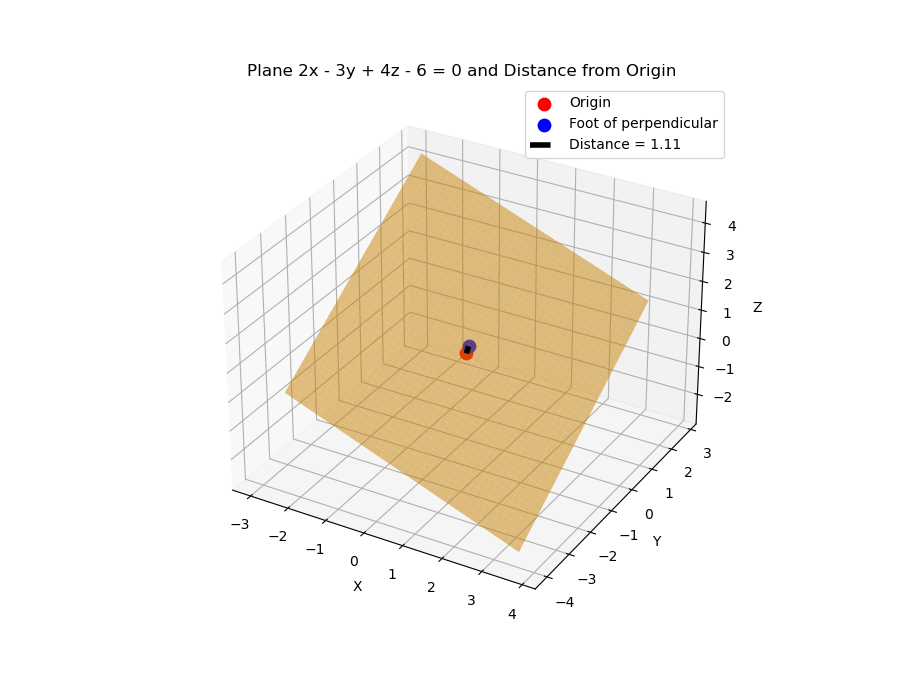
\includegraphics[width=\columnwidth, height=0.8\textheight, keepaspectratio]{Figs/fig7.png}     
\end{frame}


\begin{frame}[fragile]
\frametitle{C Code}
\begin{lstlisting}
#include <stdio.h>
#include <math.h>

int main() {
    double A = 2, B = -3, C = 4, D = -6;

    double x0 = 0, y0 = 0, z0 = 0;

    double numerator = fabs(A*x0 + B*y0 + C*z0 + D);
    double denominator = sqrt(A*A + B*B + C*C);
    double distance = numerator / denominator;

    printf("Distance of plane %.0fx + (%.0f)y + %.0fz + (%.0f) = 0 from origin is: %lf\n",
           A, B, C, D, distance);
    return 0;
}
\end{lstlisting}

\end{frame}

\begin{frame}[fragile]
\frametitle{Python and C Code}

\begin{lstlisting}

import ctypes
import numpy as np
import matplotlib.pyplot as plt

# Load the shared library
lib = ctypes.CDLL("./libdistance.so")

# Define argument and return types
lib.plane_distance.argtypes = [ctypes.c_double, ctypes.c_double,
                               ctypes.c_double, ctypes.c_double,
                               ctypes.c_double, ctypes.c_double,
                               ctypes.c_double]
lib.plane_distance.restype = ctypes.c_double

# Plane coefficients
A, B, C, D = 2, -3, 4, -6
x0, y0, z0 = 0.0, 0.0, 0.0   # origin
\end{lstlisting}

\end{frame}


\begin{frame}[fragile]
\frametitle{Python and C Code}

\begin{lstlisting}

# Call C function
dist = lib.plane_distance(A, B, C, D, x0, y0, z0)
print(f"Distance from origin = {dist:.4f}")

# ---------- PLOT ----------
# Generate grid for plane
xx, yy = np.meshgrid(np.linspace(-5, 5, 20), np.linspace(-5, 5, 20))
zz = (-A*xx - B*yy - D) / C

# Normal vector
normal = np.array([A, B, C])
normal = normal / np.linalg.norm(normal)
\end{lstlisting}

\end{frame}


\begin{frame}[fragile]
\frametitle{Python and C Code}

\begin{lstlisting}

# Closest point on plane to origin = -D * (n / |n|)
closest_point = -D * normal / (A*normal[0] + B*normal[1] + C*normal[2])

# Plot
fig = plt.figure()
ax = fig.add_subplot(111, projection='3d')

# Plane surface
ax.plot_surface(xx, yy, zz, alpha=0.5, color='cyan')

# Origin
ax.scatter([0], [0], [0], color='red', s=50, label="Origin")
\end{lstlisting}

\end{frame}


\begin{frame}[fragile]
\frametitle{Python and C Code}

\begin{lstlisting}

# Closest point
ax.scatter([closest_point[0]], [closest_point[1]], [closest_point[2]],
           color='blue', s=50, label="Closest Point")

# Distance line
ax.plot([0, closest_point[0]],
        [0, closest_point[1]],
        [0, closest_point[2]], color='black', linewidth=2)

ax.set_xlabel('X')
ax.set_ylabel('Y')
ax.set_zlabel('Z')
ax.set_title(f"Distance = {dist:.4f}")

ax.legend()
plt.show()
\end{lstlisting}

\end{frame}


\begin{frame}{Plot-Using by C and Python}
    \centering
    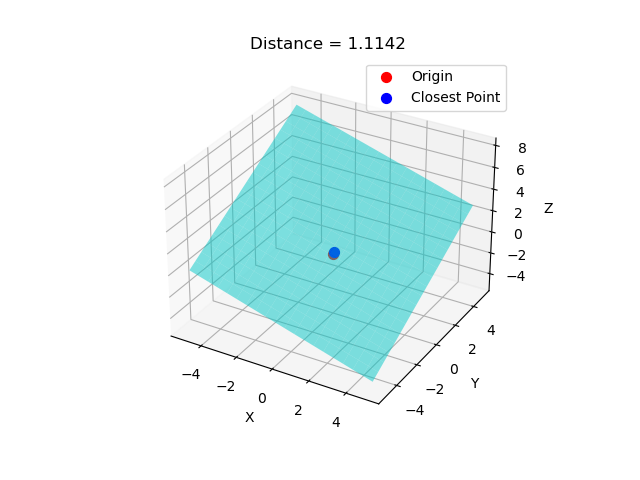
\includegraphics[width=\columnwidth, height=0.8\textheight, keepaspectratio]{Figs/Fig7.1.png}     
\end{frame}
\end{document}